\chapter{Proposed ADC Architecture}

\par
\hspace{1.2cm} The proposed architecture works based on level cross sampling scheme. Fig.~\ref{fig:PADC} shows the block diagram of the proposed ADC. Intially the sample and hold (SAH) is in sampling mode, the DAC in successive approximation ADC generates the refernce signals needed for the difference quantificator. Varition in the input analog signal crosses any of the refernce signals generated by the DAC in successive approximation ADC then difference quantificator generates conversion signal to the controller circuit and the controller circuit placeses the SAH circuit in hold mode until the conversion process is completed. Otherwise, the SAH is in sampling mode until the input anlog signal crosses any of the refence signal generated by DAC in successive approximation ADC. 

\begin{figure}[h]
	\begin{center}
		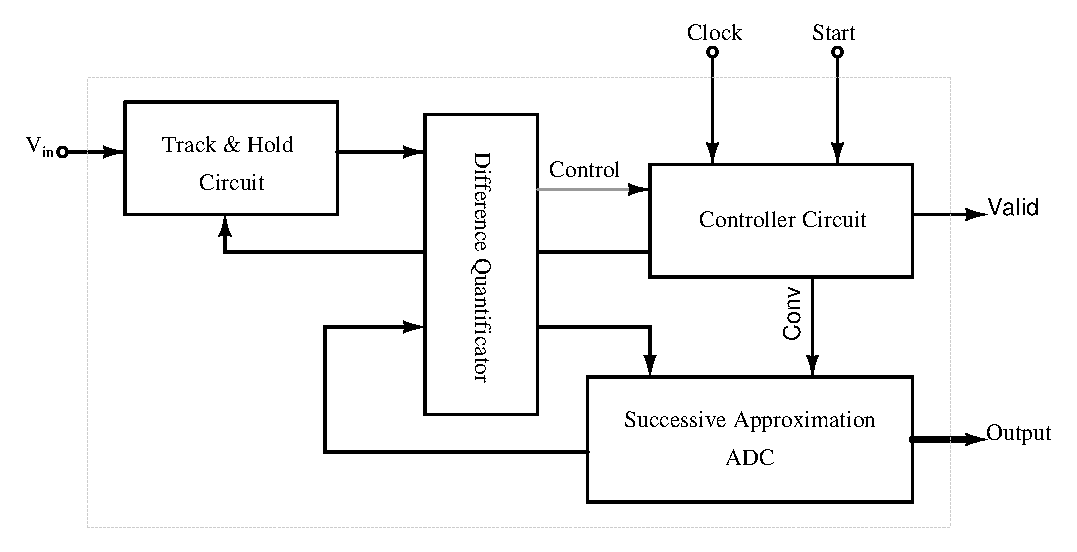
\includegraphics[scale=0.59]{./Figures/PADC.ps}
		\caption{Block Diagram of Proposed ADC}
		\label{fig:PADC}
	\end{center}
\end{figure}

\par
\hspace{0.6cm}  Controller circuit monitors the output of difference quantificator for a level crossing in the input analog signal. When the difference quantificator generates conversion signal the controller circuit generate all necessary control signals for the successive approximation ADC to convert the sampled analog signal into digital output, after completion of the conversion the analog output of the DAC is used to generate reference signal for the difference quantificator.

\par
\hspace{0.6cm} The controller circuit is also capable of loading an intial value in successive approximation register of successive approximation ADC at ever conversion process. By loading an intilligent value into successive approximation register it further decrease the number of comparisions which results in quick conversion process. Loading of intial value in successive approximation register depends on the previous ouput of the level crossing ADC and the direction in which input analog signal is traversing. Depending upon the application of level crossing ADC the contents of the successive approximation register are set from most significant bit (MSB) to least significant bit (LSB) or from LSB to MSB. A high speed counter is used to calculate the time difference between the present sample and the previous sample.

\par
\hspace{0.6cm} The proposed controller tracks the analog input in logarathmic fashion rather then linear fashion which is generally followed in conventional level crossing ADC's. At maximum the proposed level crossing ADC takes $2N$ clock cycles for complete the process in low frequency applications and $N$ clock cycles for high frequency applications. Where as in convetional  level crossing ADC's which use up-down counter will take $2^N$ clock cycles to complete the operation when the analog input changes from minimum to maximum value. Further the controller circuit can be programmed for low frequency applications in such a way that the maximum number of clock cycles required to convert input analog signal when changing from minimum to maximum can range in between $N$ to $2N$, where $N$ is the number of bits in level crossing ADC.\par


\section{Controller for high frequency applications}

\par
\hspace{1.2cm} In high frequency applications the input analog signal varies very rapidly. So, the bits in successive approximation register are set from the MSB to LSB. Some of the bits in the successive approximation register can be retained depending on the direction of the input analog signal traversing and the previous output of the level crossing ADC. The number of bits retained is same as the number of comparisions not needed to evaluate the present sampled analog signal which required to convert into digital output. The operation of controller circuit for high frequency applicatons is shown in Fig.~\ref{fig:HFA} as a flow chart for 8-bit hardwear resolution. \par


\par
\hspace{0.6cm} When the analog input signal is increasing then the present level crossing ADC output should be larger than the previous level crossing ADC output. So, all comparisons which results in present level crossing ADC output less than compared to previous level crossing ADC output can be eliminated. Similarly, when the analog input signal is decreasing then the present level crossing ADC output should be less then the previous level crossing ADC output. So, all coaprisons which results in present level crossing ADC output greater than compared to previous level crossing ADC Can be eliminated. The above situtions translated into the following process when setting the intial value into the successive approximation register.

\begin{figure}[H]
	\begin{center}
		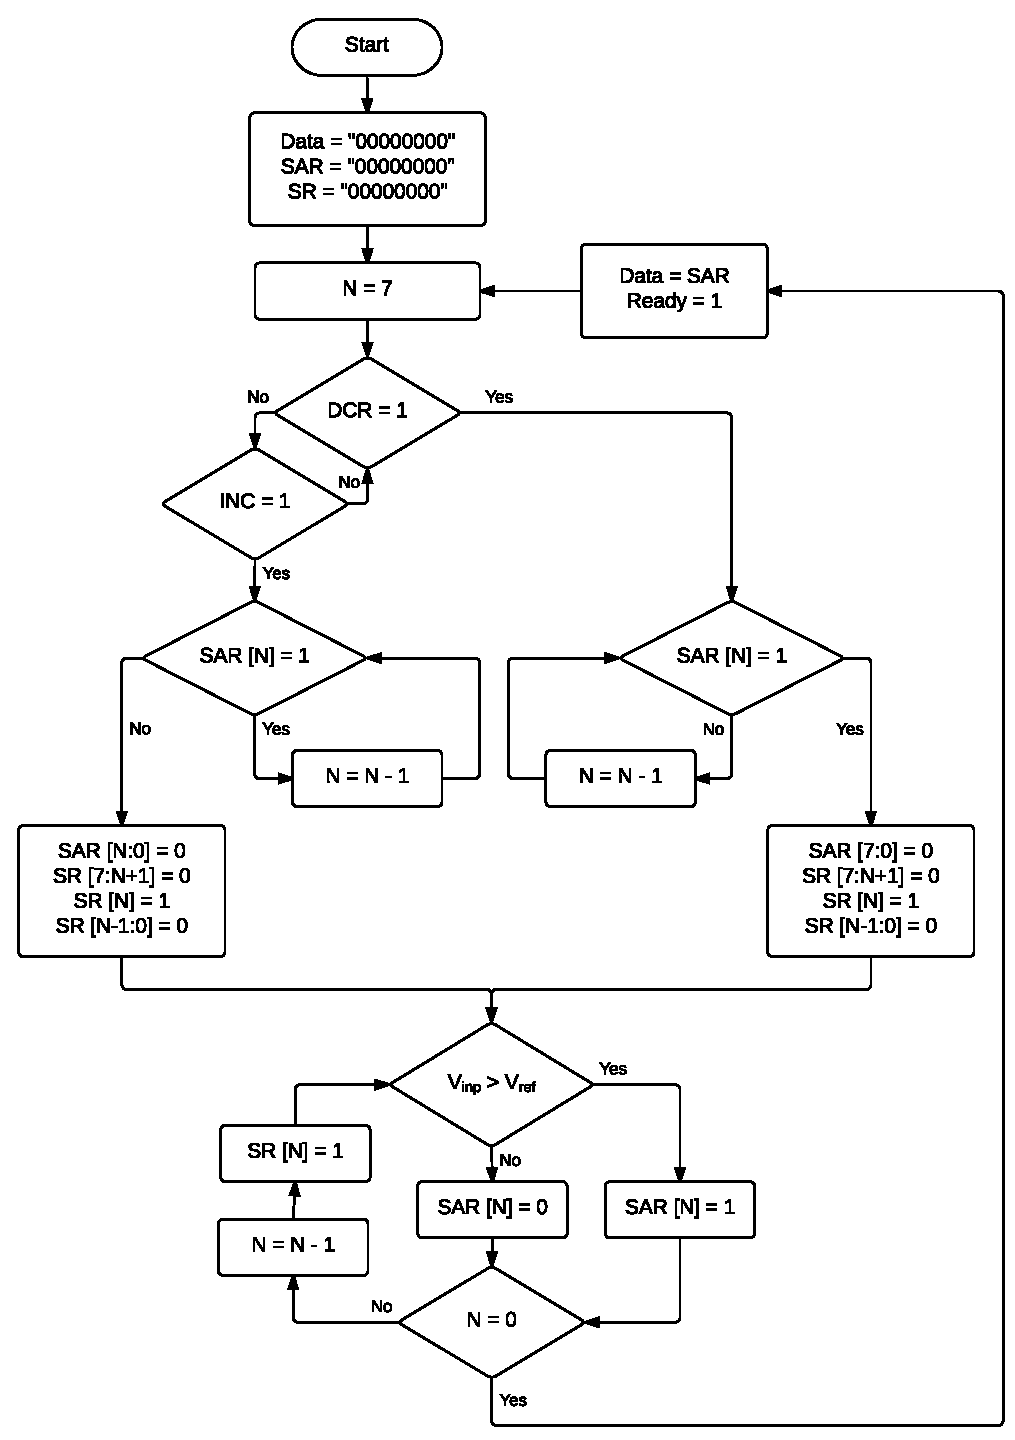
\includegraphics[width=10.1 cm, angle=360]{./Figures/HFA.ps}
		\caption{Controller operation for high frequency applications}
		\label{fig:HFA}
	\end{center}
\end{figure}

\par
\hspace{0.6cm} If the input analog signal is increasing the successive approximation register is assigned with all MS bits to '1' until first '0' and remaining bits are set to '0'. Shift Register is assigned with with all '0' except the first '0' in successive approximation register bit is set to '1'. If the input signal is decreasing the successive approximation register is assigned with all bits set to '0'. Shift Register is assigned with with all '0' except the first '1' in successive approximation register bit is set to '1'. Following examples demonstrates the situation for the proposed level crossing ADC to reduce the activity of the conversion circuit for high frequency applications. Fig.~\ref{fig:MHF} shows the Matlab result for reduction in activity with respect to the binary code for both the cases when the input analog signal is increasing and decreasing.

\par
\hspace{0.6cm}\textbf{Example 1}: When analog input is increasing if contents of successive approximation register are $11010110$, then value assigned to Shift Register is $00100000$ and value assigned to successive approximation register is $11000000$, which results reduction in two comparison states.

\begin{table}[h]		
	\begin{center}	
		\begin{tabular}{ c  c  c  c  c  c  c  c  c }
					Shift Reg  	& 0 & 0 & \textbf{1} & 0 & 0 & 0 & 0 & 0 \\
				   				&  &  & $\Uparrow$ & & & & & \\		
	 				\textbf{Output}   & \textbf{1} & \textbf{1} & \textbf{0} & 0 & 1 & 1 & 1 & 0 \\
				   				& $\Downarrow$ & $\Downarrow$ & & & & & & \\
					SA Reg     	& \textbf{1} & \textbf{1} & 0 & 0 & 0 & 0 & 0 & 0 \\			
		\end{tabular}
	\end{center}
\end{table}

\par
\hspace{0.6cm}\textbf{Example 2}: When analog input is decreasing if contents of successive approximation register are  $00010110$, then value assigned to Shift Register is $00010000$ and value assigned to successive approximation register is $00000000$, which results reduction in two comparison states.

\begin{table}[h]
\begin{center}	
		\begin{tabular}{ c  c  c  c  c  c  c  c  c }
					Shift Reg  	& 0 & 0 & 0 & 0 & \textbf{1} & 0 & 0 & 0 \\
				   				& &  &  &  &$\Uparrow$ & & & \\	
	 		 		\textbf{Output}   & \textbf{0} & \textbf{0} & \textbf{0} & \textbf{0} & \textbf{1} & 1 & 1 & 0 \\
				   				& $\Downarrow$ & $\Downarrow$ &  $\Downarrow$ &  $\Downarrow$ & & & & \\
					SA Reg     	& \textbf{0} & \textbf{0} & \textbf{0} & \textbf{0} & 0 & 0 & 0 & 0 \\
			
		\end{tabular}
	\end{center}
\end{table}

\begin{figure}[H]
	\begin{center}
		\includegraphics[scale=0.4]{./Figures/FAST.eps}
		\caption{Reduction in activity with digital code}
		\label{fig:MHF}
	\end{center}
\end{figure}



\section{Controller for low frequency applications}

\par
\hspace{1.2cm} In low frequency applications the input analog signal varies slowly. So, the bits in successive approximation register are set from the LSB to MSB. Some of the bits in the successive approximation register can be retained depending on the direction of the input analog signal traversing and the previous output of the level crossing ADC. The operation of controller for low frequency applicatons is shown in Fig.~\ref{fig:LFA} as a flow chart for 8-bit hardwear resolution. \par

\begin{figure}[H]
	\begin{center}
		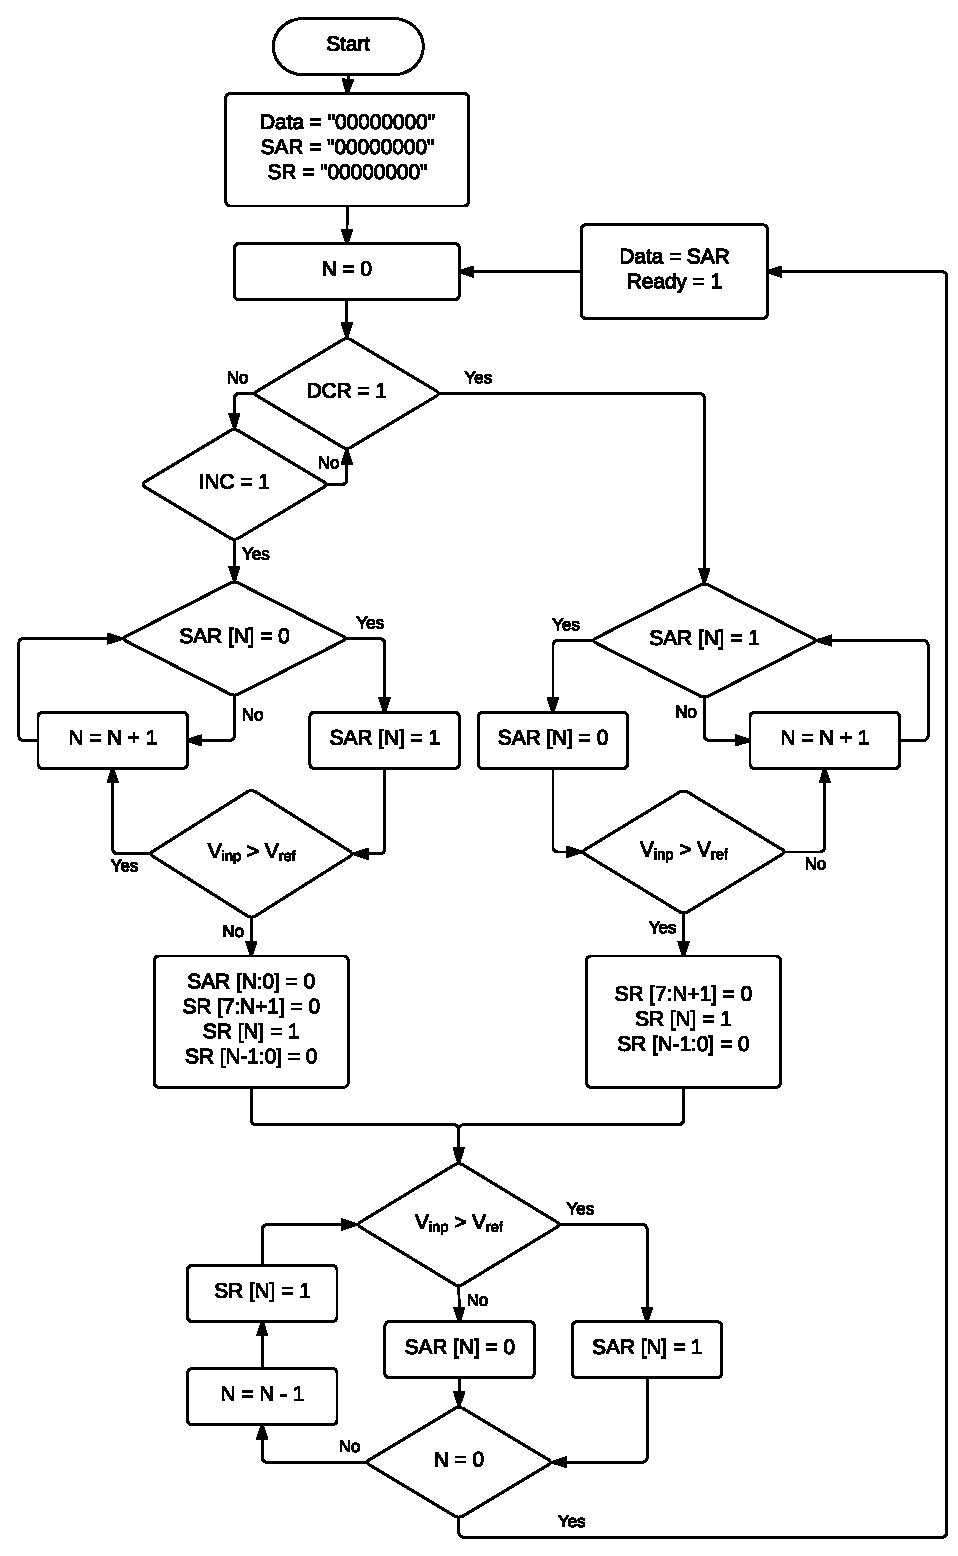
\includegraphics[width=9.8 cm, angle=360]{./Figures/LFA.ps}
		\caption{Controller operation for low frequency applications}
		\label{fig:LFA}
	\end{center}
\end{figure}

\par
\hspace{0.6cm} The controller circuit works in two phases for both the cases when input analog signal increasing or decreasing. In first phase it checks for the vilation of the obtained condition and in the second phase it estimates the exact value of the sampled analog signal. In first phase when the input analog signal is increasing then the '0's from LSB will be converted into '1's one by one and checking whether the resulting signal is greater than input analog signal. until the case is achieved all bits from LSB to MSB are converted to 1's. When the condition is reached all the MSB bits are copied as they are upto the current bit and all remaing bits are assigned with zeros in successive approximation register. The shift register is loaded with all zeros except the bit when the condition is achieved is made one and then normal sucessive approximation conversion process is folled. 

\par
\hspace{0.6cm} Similarly, when the input analog signal is decreasing then the 1's from LSB will be converted into 0's one by one and checking whether the resulting signal is less than input analog signal. Until this condition is achieved all bits from LSB to MSB are converted to 0's. When the condition is reached all the MSB bits are copied as they are upto the curren bit and all remaining bits are assigned with zeros in successive approximation register. the shift register is loaded with all zeros except the bit when the condition is achieved is made one and then normal successive approximation process is followed to finad the exact value of the sampled analog signal.   

\par
\hspace{0.6cm} Following examples demonstrates the situation for the proposed level crossing ADC to reduce the activity of the conversion circuit for high frequency applications. Fig.~\ref{fig:MHF} shows the Matlab result for reduction in activity with respect to the binary code for both the cases when the input analog signal is increasing and decreasing.

\begin{figure}[H]
	\begin{center}
		\includegraphics[scale=0.4]{./Figures/SLOW.eps}
		\caption{Reduction in activity with digital code}
		\label{fig:MLF}
	\end{center}
\end{figure}


